\chapter{INTRODUÇÃO}

\section{Contextualização}

Nos tempos atuais, a evolução tecnológica recente tem sido orientada pela crescente e constante demanda por aplicações \textit{web} mais rápidas, escaláveis e confiáveis. Nesse sentido, a comunicação entre sistemas distribuídos passou a ganhar espaço próprio, sobretudo em razão da expansão de serviços digitais, plataformas \textit{online} e aplicações em nuvem. Assim, a eficiência da troca de informações entre clientes e servidores passou a afetar diretamente a experiência do usuário e o desempenho desses sistemas.

Neste cenário, as \textit{Application}\textit{ }\textit{Programming}\textit{ Interfaces} (APIs) se tornaram um dos principais meios de integração entre sistemas. A popularização dessas arquiteturas baseadas em serviços, como microsserviços, ampliou a necessidade de protocolos capazes de lidar com grandes volumes de requisições e de manter baixa latência nas respostas (TRIPATHI; MIRAZ; JOSHI, 2023).

Essas demandas têm sido acompanhadas dos protocolos de comunicação web, cuja evolução é crescente diante das novas versões voltadas a desempenho, segurança e confiabilidade. Contudo, a adoção dessas inovações nem sempre chega de imediato aos ambientes de desenvolvimento mais utilizados, o que levanta questões sobre sua viabilidade prática e sobre os desafios de implementação (KOCH; FALOWO; ELROD, 2024).

\section{Problema investigado}

Entre as novas versões de protocolos \textit{web}, destaca-se o HTTP/3, que altera substancialmente o modo com que a comunicação é estabelecida ao adotar o QUIC sobre UDP como transporte (QUIC Working Group - IETF, 2021; IETF, 2022). Entretanto, os benefícios a ele relacionados, como a redução de latência e maior resiliência em redes instáveis, ainda não chegaram de forma efetiva a ambientes consolidados no desenvolvimento \textit{web}, como no caso do Node.js, o qual não oferece suporte nativo estável ao protocolo (KOCH; FALOWO; ELROD, 2024).

Essa limitação evidencia, assim, uma lacuna entre a evolução dos protocolos e sua adoção prática em ecossistemas utilizados amplamente. Deste cenário, emergem questionamentos acerca da viabilidade do HTTP/3 em aplicações reais, especialmente em projetos que se utilizam de \textit{frameworks} populares e que dependem de infraestruturas intermediárias, como \textit{proxies} reversos e \textit{gateways} (TRIPATHI; MIRAZ; JOSHI, 2023).

Logo, este trabalho visa investigar o problema de incorporação do HTTP/3, sobretudo em contextos os quais não foram projetados para suportá-lo, destacando quais os desafios técnicos, as limitações e as estratégias possíveis para viabilizar a sua adoção em aplicações baseadas em Node.js.

\section{Motivação}

O HTTP persiste como o principal canal de comunicação na \textit{web}, de modo que o HTTP/3 sobre QUIC representa um avanço adicional no que tange a desempenho e a resiliência em redes adversas (PERNA et al., 2022; QUIC Working Group - IETF, 2021). No Node.js, entretanto, essa evolução ainda carece de meios alternativos de viabilização da integração. Surge, assim, a motivação do presente trabalho, a qual advém da necessidade de examinar justamente essa transição em APIs REST - um cenário típico de microsserviços - no qual definir quando e como expor o HTTP/3 sem reescrever o \textit{backend} representa um desafio prático para as equipes de desenvolvimento.

\section{Objetivo}

Objetiva-se, pois, com este trabalho, examinar a viabilidade, os desafios, o desempenho comparativo e as estratégias de integração do HTTP/3 em APIs REST baseadas em Node.js, articulando fundamentação teórica, revisão rápida da literatura e, especialmente, o estudo de caso experimental. Nele, foi desenvolvida uma API orientada a benchmarks, exposta a HTTP/1.1, HTTP/2 e HTTP/3 com terminação QUIC em proxy reverso NGINX; cujos resultados serão analisados nos Capítulos 4 e 5.

\subsection{Objetivos específicos}

Com base no objetivo geral, este trabalho persegue os seguintes objetivos específicos:

\begin{enumerate}[label=\alph*)]
\item verificar a viabilidade de expor HTTP/3 a APIs Node.js sem suporte nativo estável ao protocolo, por meio de proxy reverso;
\item identificar e documentar os principais desafios técnicos e operacionais da adoção de HTTP/3 nesse contexto;
\item comparar quantitativamente o desempenho de HTTP/1.1, HTTP/2 e HTTP/3 em cenários controlados de carga, payload e rede;
\item construir e disponibilizar um artefato reprodutível que materialize estratégias de integração em ambientes já consolidados.
\end{enumerate}

\section{Metodologia}

Este trabalho se baseia em uma abordagem experimental, através da combinação de uma revisão teórica e da validação prática. A Figura 1 resume as etapas executadas.

\begin{figure}[H]
\centering
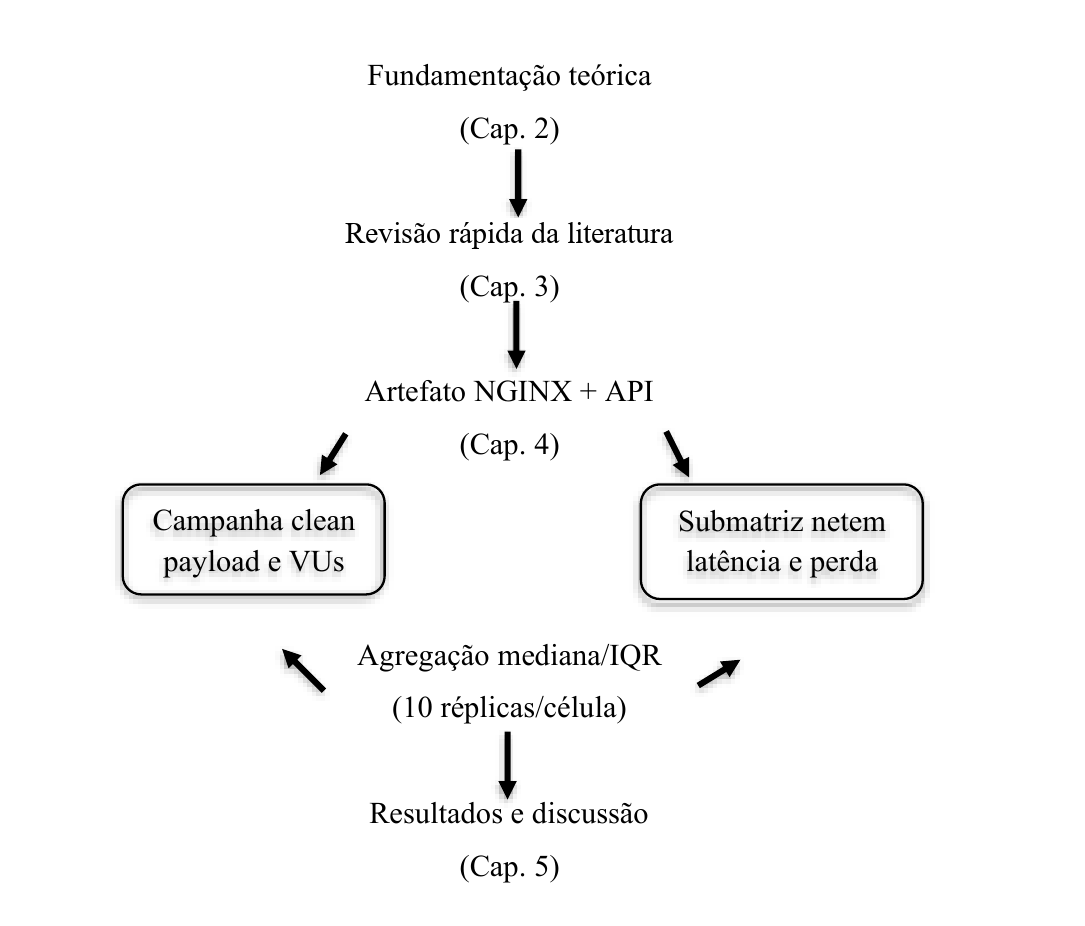
\includegraphics[width=0.92\textwidth]{assets/figuras/fig1.png}
\caption{Fluxo metodológico do trabalho}
\fonte{Fonte: elaborado pelo autor}
\end{figure}

No que tange ao eixo teórico, o Capítulo 2 busca apresentar a fundamentação sobre HTTP, QUIC e HTTP/3, Node.js, APIs REST e métricas de desempenho; enquanto o Capítulo 3 conduz a revisão rápida da literatura (KITCHENHAM; CHARTERS, 2007; CARTAXO; PINTO; SOARES, 2020), com protocolo de busca, critérios de inclusão e síntese temática.

Já em relação ao eixo prático, foi implementado um artefato reprodutível (API Node.js, NGINX, Docker e roteiros de coleta) descrito no Capítulo 4. O HTTP/3 é exposto na borda por proxy reverso, pois o \textit{runtime} não oferece suporte nativo estável ao protocolo (KOCH; FALOWO; ELROD, 2024).

As campanhas de carga utilizam k6 para HTTP/1.1 e HTTP/2 e cliente QUIC dedicado para HTTP/3, em matriz clean (variação de payload e concorrência) e submatriz com tc netem (perfis de latência e perda). Cada célula reportada resume dez réplicas pela mediana e pelo intervalo interquartil (IQR). A análise comparativa e as ameaças à validade estão representadas no Capítulo 5.

\section{Justificativa}

Tendo-se em vista que a evolução dos protocolos \textit{web} exige que equipes de desenvolvimento compreendam como integrar HTTP/3 em stacks já consolidadas, sem reescrever aplicações inteiras, este trabalho se justifica pela reunião de evidências bibliográficas e empíricas acerca do desempenho e da migração em APIs REST (PERNA et al., 2022; TRIPATHI; MIRAZ; JOSHI, 2023; MUÑOZ et al., 2025), além de disponibilizar artefato e roteiros reprodutíveis que apoiam decisões técnicas e pesquisas posteriores sobre Node.js e proxy reverso. 

\section{Contribuições}

Este trabalho visa contribuir com uma revisão rápida da literatura sobre HTTP/3, QUIC e APIs REST, destacando lacunas quanto a Node.js e proxy reverso, mas também com um artefato de software reprodutível (API, infraestrutura Docker/NGINX e roteiros de benchmark), o qual permite investigar empiricamente essa lacuna. Também, contribui com a apresentação de evidências empíricas comparativas entre HTTP/1.1, HTTP/2 e HTTP/3, com agregação estatística e com a discussão de limitações metodológicas, disponibilizadas em repositório aberto para replicação.

\section{Questões de pesquisa}

Com base no problema investigado, este trabalho busca responder às seguintes questões de pesquisa:

\begin{enumerate}[label=\alph*)]
\item é viável utilizar o protocolo HTTP/3 em aplicações desenvolvidas com Node.js, mesmo na ausência de suporte nativo estável?
\item quais são os principais desafios técnicos envolvidos na adoção do HTTP/3 nesse contexto?
\item como o desempenho de aplicações utilizando HTTP/3 se compara às versões anteriores do protocolo, como HTTP/1.1 e HTTP/2?
\item quais estratégias podem ser utilizadas para viabilizar a integração do HTTP/3 em ambientes já consolidados?
\end{enumerate}

\section{Delimitação do Estudo}

Este estudo se concentra na análise da viabilidade de utilização do protocolo HTTP/3 em aplicações \textit{backend} desenvolvidas com Node.js, com enfoque específico em APIs REST e em testes de desempenho. A investigação limita-se à avaliação de métricas como latência, tempo de resposta, TTFB, taxa de transferência e comportamento sob carga.

Nesse sentido, não compõem o escopo do trabalho aspectos de \textit{frontend}, experiência do usuário final ou implantação em produção em larga escala. Implementações nativas de HTTP/3 em outras linguagens ou plataformas também ficam fora do recorte, o qual se restringe ao ecossistema Node.js.

O HTTP/3 foi avaliado por meio de proxy reverso e servidores intermediários, sem modificações no núcleo do Node.js. Os resultados refletem cenário controlado de laboratório e podem não abranger todas as variáveis de ambientes produtivos.

